\documentclass[a4paper,10pt,ngerman]{scrartcl}
\usepackage{babel}
\usepackage[T1]{fontenc}
\usepackage[utf8x]{inputenc}
\usepackage[a4paper,margin=2.5cm,footskip=0.5cm]{geometry}
\usepackage{listings}

\newcommand{\Aufgabe}{Aufgabe 1: Hopsitexte}
\newcommand{\TeamId}{00178}
\newcommand{\TeamName}{Team-Name}
\newcommand{\Namen}{Matthew Greiner}
 
% Kopf- und Fußzeilen
\usepackage{scrlayer-scrpage, lastpage}
\setkomafont{pageheadfoot}{\large\textrm}
\lohead{\Aufgabe}
\rohead{Team-ID: \TeamId}
\cfoot*{\thepage{}/\pageref{LastPage}}

\lstset{
    literate={ä}{{\"a}}1
             {ö}{{\"o}}1
             {ü}{{\"u}}1
             {Ä}{{\"A}}1
             {Ö}{{\"O}}1
             {Ü}{{\"U}}1
             {ß}{{\ss}}1
}

\lstset{ %
  language=Java,
  basicstyle=\ttfamily\small,
  keywordstyle=\color{blue},
  commentstyle=\color{green!50!black},
  stringstyle=\color{orange},
  numbers=left,
  numberstyle=\tiny\color{gray},
  stepnumber=1,
  numbersep=5pt,
  backgroundcolor=\color{white},
  showspaces=false,
  showstringspaces=false,
  tabsize=2,
  breaklines=true,
  breakatwhitespace=true,
  frame=single,
  captionpos=b,
}

% Position des Titels
\usepackage{titling}
\setlength{\droptitle}{-1.0cm}

% Für mathematische Befehle und Symbole
\usepackage{amsmath}
\usepackage{amssymb}

% Für Bilder
\usepackage{graphicx}
\graphicspath{ {./bilder/} }

% Für Algorithmen
\usepackage{algpseudocode}

% Für Quelltext
\usepackage{listings}
\usepackage{color}
\definecolor{mygreen}{rgb}{0,0.6,0}
\definecolor{mygray}{rgb}{0.5,0.5,0.5}
\definecolor{mymauve}{rgb}{0.58,0,0.82}
\lstset{
  keywordstyle=\color{blue},commentstyle=\color{mygreen},
  stringstyle=\color{mymauve},rulecolor=\color{black},
  basicstyle=\footnotesize\ttfamily,numberstyle=\tiny\color{mygray},
  captionpos=b, % sets the caption-position to bottom
  keepspaces=true, % keeps spaces in text
  numbers=left, numbersep=5pt, showspaces=false,showstringspaces=true,
  showtabs=false, stepnumber=2, tabsize=2, title=\lstname
}
\lstdefinelanguage{JavaScript}{ % JavaScript ist als einzige Sprache noch nicht vordefiniert
  keywords={break, case, catch, continue, debugger, default, delete, do, else, finally, for, function, if, in, instanceof, new, return, switch, this, throw, try, typeof, var, void, while, with},
  morecomment=[l]{//},
  morecomment=[s]{/*}{*/},
  morestring=[b]',
  morestring=[b]",
  sensitive=true
}

% Diese beiden Pakete müssen zuletzt geladen werden
%\usepackage{hyperref} % Anklickbare Links im Dokument
\usepackage{cleveref}

% Daten für die Titelseite
\title{\textbf{\Huge\Aufgabe}}
\author{\LARGE Team-ID: \LARGE \TeamId \\\\
	    \LARGE Team-Name: \LARGE \TeamName \\\\
	    \LARGE Bearbeiter/-innen dieser Aufgabe: \\ 
	    \LARGE \Namen\\\\}
\date{\LARGE\today}

\begin{document}

\maketitle
\tableofcontents

\vspace{0.5cm}

\section{Lösungsidee / Ansatz}
\subsection{Anforderungen an das Programm}
In dieser Aufgabe geht es darum, ein Programm zu erstellen, das Zara hilft, deutsche Hopsitexte zu erstellen. 
Um ein Programm zu gestalten, damit Zara besonders gut damit arbeiten kann, müssen meiner Meinung nach folgende Kriterien für das Programm erfühlt sein: 
\begin{itemize}
    \item[1.]Das Programm muss ein graphisches Nutzerinterface mit einem Textfeld haben, in der Zara ihren Text tippen kann.
    \item[2.]Die Stellen, an denen die Sprünge stattgefunden haben, müssen wie in den Beispieltexten, rot für den ersten Spieler und blau für den zweiten Spieler, gefärbt sein.
    \item[3.]Da es ein deutscher Text sein soll, müssen Umlaute wie "ä, ö, ü" und "ß" auch unterstützt werden.
    \item[4.]Wenn der Text kein Hopsitext ist, muss die Stelle, an dem sich die Spieler treffen, farblich markiert sein, damit Zara merkt, dass sie Änderungen vornehmen muss.
    \item[5.]Es muss anzeigen, ob der eingegebene Text ein "Hopsitext" ist oder nicht.
    \item[6.]Die Ausgabe des Programmes und die farbliche Markierungen des Eingabetextes muss dynamisch und automatisch mit dem Tippen von Zara geschehen und Zara kann an beliebigen Stellen im Eingabetext Änderungen vornehmen (Quality of life).
\end{itemize}
Auf der linken Seite des Programmes soll Zara ihren Text tippen können und auf der rechten Seite soll dieser Text, an den Sprüngen der Spieler farblich markiert - wie im Beispieltext, angezeigt werden.
So sieht Zara beim tippen, ob ihre aktuelle Eingabe ein Hopsitext ist oder nicht. Zusätzlich soll oberhalb des Textfeldes deutlich angezeigt werden, ob es sich um einen Hopsitext handelt.
Wenn diese Kriterien erfüllt sind, hat Zara ein Programm, in der sie einen Text schreiben kann, das ihr beim tippen anzeigt, ob ihre aktuelle Eingabe ein Hopsitext ist oder nicht. Falls es kein Hopsitext ist, sieht Zara das sofort und kann ihren Text bzw. einfach die letzen Worte mit dem Sprung, ändern.

\section{Umsetzung}
Um dieses Programm zu erstellen, habe ich JavaFX als GUI Library verwenden, welches mir grundlegende Bausteine für das Interface zur Verfügung stellt. Zur Implementierung werden die in \text{1.1} angesprochenen Anforderungen einzeln umgesetzt:

\begin{itemize}
  \item [1.] Zu Begin erstelle ich mit Modulen ein Textfeld ("TextArea") auf der linken Seite des Programms, eine formatierte Textanzeige ("Textflow") auf der rechten Seite, in der die Hopsisprünge markiert werden und einen Statustext ("Text") mit dem Ergebnis ganz oben.
  Das Textfeld bekommt einen Listener, der jedes mal gerufen wird, wenn sich der Text im Textfeld ändert. So wird jedes mal das Ergebnis und der formatierte Text auf der rechten Seite geupdated, sobald sich die Texteingabe ändert.
  \item [2.] Eine Methode die die Texthops-Regeln beginnend an einer Startposition simuliert, muss erstellt werden. Diese Methode wird zweimal aufgerufen, jeweils einmal für die Roten und die Blauen Sprünge. Die Methode funktioniert wie folgt:
  \begin{itemize}
    \item [1.] Der Eingabetext wird als String und die Farbe, mit der gesprungen werden soll, wird übergeben.
    \item [2.] Die ersten nicht Zeichen, die keine Buchstaben sind werden bei der Simulation der Texthops-regeln übersprungen und bei dem ersten Zeichen, das ein Buchstabe ist, wird begonnen.
    \item [3.] Dieses Zeichen wird mit der übergebenen Farbe gefärbt und zu einer Collection aus Zeichen (TextFlow) hinzugefügt. Die Position des Buchstabens im Alphabet wird sich gemerkt; z.B. als $n$.
    \item [4.] Dann werden die nächsten $n$ Buchstaben übersprungen. Alle Zeichen, die keine Buchstaben sind, werden ignoriert. Alle Zeichen, inklusive der Nicht-Buchstaben werden ungefärbt zu dem TextFlow hinzugefügt.
    \item [5.] Anschließend wird der Buchstabe bei dem wir nach den Sprüngen angekommen sind, mit der übergeben Farbe gefärbt und zum Textflow hinzugefügt. Diese Schleife (3. - 5.) wird wiederholt, bis der Inputtext vollständig geparst wurde.
    \item [6.] Das resultierende TextFlow enthält nun den gesamten Inputtext, wobei die Hopsisprünge farblich markiert sind. Dieses Textflow wird zurückgegeben.
  \end{itemize}
  \item [3.] Um die Sprungweite eines Buchstabens gleich weit wie ihre Position im Alphabet zu machen und Umlaute auch zu beachten, muss eine Methode erstellt werden, die die zugehörige Sprungweite von einem übergebenen Zeichen zurückgibt:
  Wenn das übergebene Zeichen ein deutsches Sonderzeichen ist, wird eine festgelegt Position zurückgegeben. Wenn es sich um einen normalen kleinen Buchstaben handelt, kann man um die Position im Alphabet zu bekommen, den ASCII-Wert dem Zeichen mit dem ASCII-Wert von "A" subtrahieren und 1 addieren. So ist A=1, B=2, etc.
  Kleinbuchstaben funktionieren analog, nur wird hier der ASCII-Wert von "a" abgezogen. Alle anderen Zeichen geben -1 zurück.
  \item[4.] Um die Stelle, bei der sich beide Spieler treffen, farblich zu markieren (z.B. \textbf{lila}), muss die Methode von (2.) verwendet werden. Diese wird verwendet, um die Sprünge von beiden Spielern zu berechnen und in einem TextFlow farblich zu markieren.
  Nun müssen diese beiden TextFlows verglichen werden, und wenn an einer Stelle des Texts, der Buchstabe in beiden TextFlows farblich markiert sind, treffen sich die beiden Spieler hier. Daher muss für dieses Teilproblem eine Methode erstellt werden, die diese beiden TextFlows mit den einzelnen Sprüngen vereinigt und 
  wenn sich die Spieler treffen, farblich markiert (lila), und dies als Ergebnis dem Nutzer anzeigt.
  \item[5.] Wenn die Methode aus (4.) an beliebiger Stelle lila anzeigt, ist der übergebenen Text kein Hopsitext mehr. Dies wir über dem Nutzereingabefeld bekenntlich gemacht.
  \item[6.] Das von oben genannte wird jedes mal ausführt, wenn sich das Eingabefeld ändert.
\end{itemize}

\newpage

\section{Beispiele}
\subsection{Beispiele BwInf-Aufgabenangaben}
Hier ist das Progamm mit den Angabetexten der Junioraufgabe 2 und der Aufgabe 1 als Eingabetext.
\newline

\textbf{Angabe aus Junioraufgabe 2}
\newline

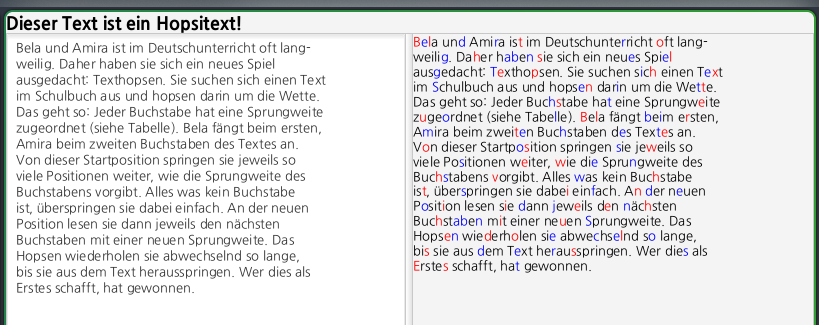
\includegraphics[scale=0.55]{junioraufgabe2-eingabe.png}
\newline

\textbf{Angabe aus Aufgabe 1}
\newline

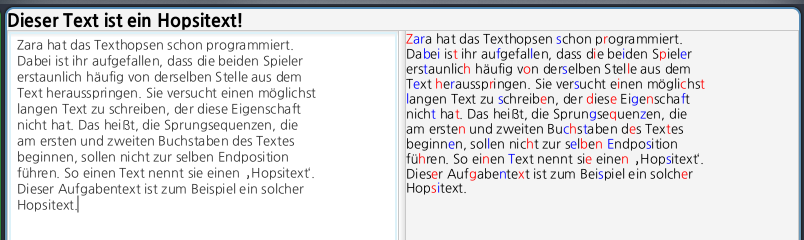
\includegraphics[scale=0.55]{aufgabe1-angabe.png}

\subsection{Eigene Beispiele / Edgecases}

\textbf{Kurze Texte}
\newline
\newline
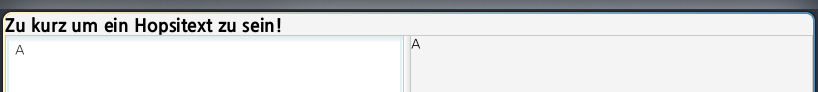
\includegraphics[scale=0.55]{kurz1.png}
\newline
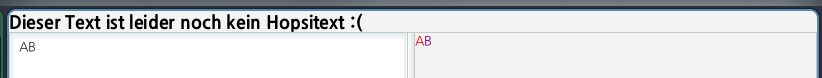
\includegraphics[scale=0.55]{kurz2.png}
\newline
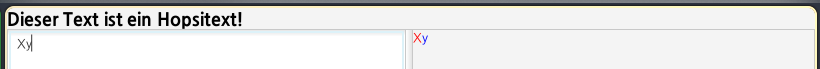
\includegraphics[scale=0.55]{kurz3.png}

\newpage
\textbf{Random Input}
\newline
\newline
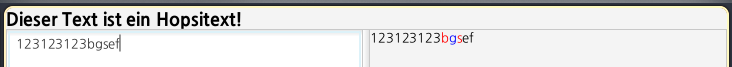
\includegraphics[scale=0.60]{rand1.png}
\newline
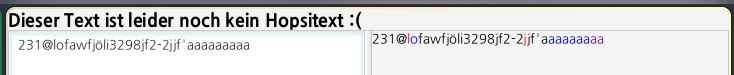
\includegraphics[scale=0.60]{rand2.png}
\newline
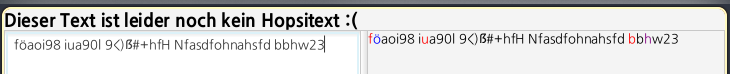
\includegraphics[scale=0.60]{rand3.png}
\newline
\newline

\textbf{Lange Texte}
\newline
\newline
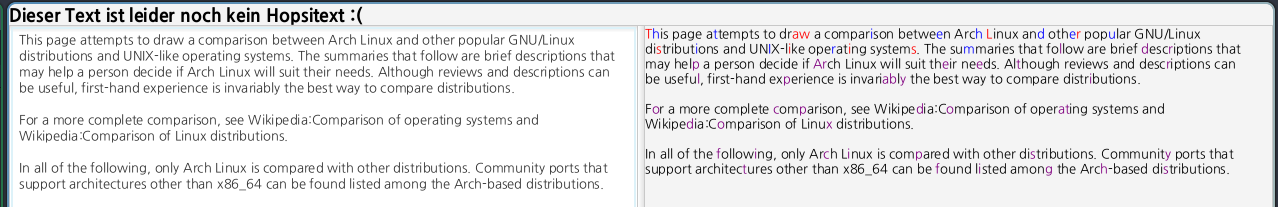
\includegraphics[scale=0.35]{lang1.png}
\newline
\newline
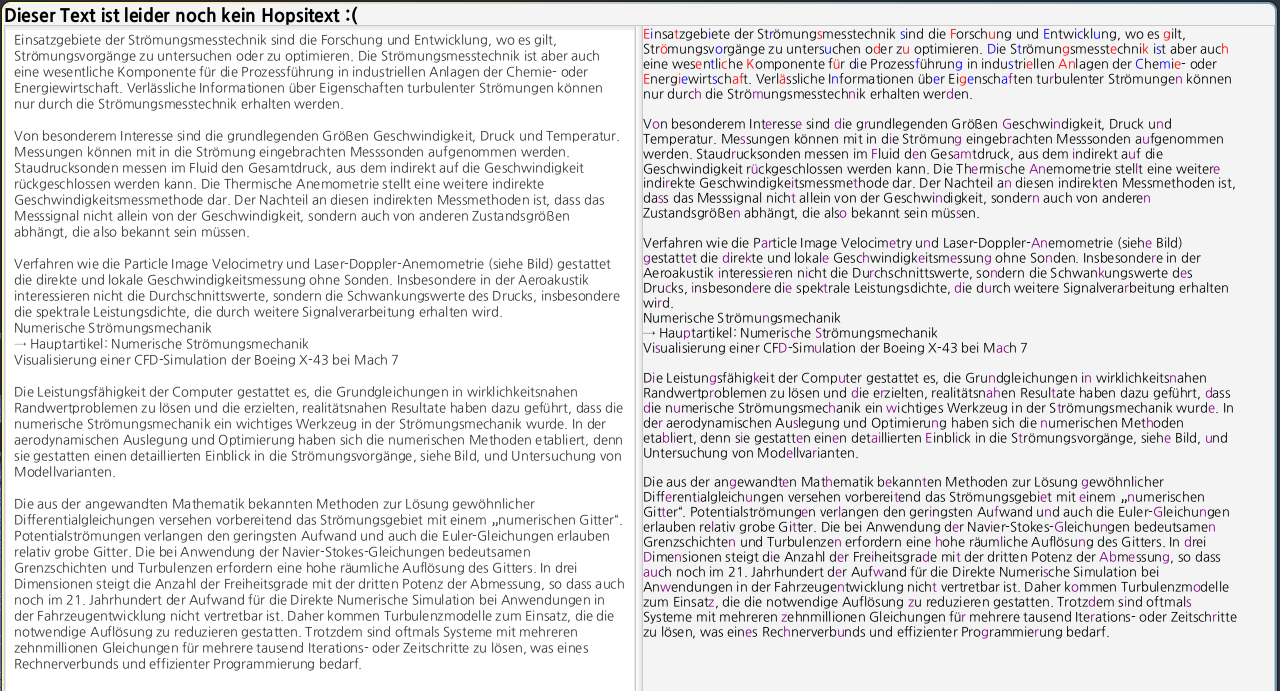
\includegraphics[scale=0.35]{lang2.png}

\newpage
\section{Quellcode}
\textbf{Simuliert Hopsitext Sprünge - Entspricht der Methode aus (2.2)}
\newline
\begin{lstlisting}
/** 
* Simulates Hopsitext-jumps
* 
* @param input - Inputtext as String
* @param startIndex - Starting Position of Player
* @param color - Color of Player
* @return TextFlow
*/
private TextFlow jump(String input, int startIndex, Color color) {
    // Textflow is a collection of textnodes
    TextFlow tf = new TextFlow();
    int nextIndex = 0;
    char currentChar = ' ';
    // Textnode is a single character, because characters need to be colored
    // individually
    Text textNode = new Text();

    // Skip over first non-alphabetic characters
    int i = 0;
    for (; i < input.length(); i++) {
        if (getAlphabetPosition(input.charAt(nextIndex)) == -1) {
            textNode = new Text(String.valueOf(input.charAt(nextIndex)));
            tf.getChildren().add(textNode);
            nextIndex++;
        } else {
            break;
        }
    }
    nextIndex += startIndex;

    if (nextIndex == (1 + i) && !input.isEmpty()) {
        textNode = new Text(String.valueOf(input.charAt(0)));
        tf.getChildren().add(textNode);
    }

    // Main loop
    while (nextIndex < input.length()) {
        currentChar = input.charAt(nextIndex);
        textNode = new Text(String.valueOf(currentChar));

        // Character that needs to be colored, beause jump starts on this char
        if (getAlphabetPosition(currentChar) != -1) {
            // Display character in specified color
            textNode.setFill(color);
            tf.getChildren().add(textNode);

            int alphabetPosition = getAlphabetPosition(currentChar);
            int count = 0;

            // Skip non-alphabetic characters and move forward by the alphabet position
            while (count < alphabetPosition) {
                nextIndex++;
                if (nextIndex >= input.length()) {
                    break;
                }
                // If Character is an alphabetic character
                if (getAlphabetPosition(input.charAt(nextIndex)) != -1) {
                    count++;
                    // Add uncolored character
                    if (count != alphabetPosition) {
                        textNode = new Text(String.valueOf(input.charAt(nextIndex)));
                        tf.getChildren().add(textNode);
                    }
                    // If Character is non alphabetic -> skip it and don't increment loop counter
                } else {
                    // Add uncolored character
                    textNode = new Text(String.valueOf(input.charAt(nextIndex)));
                    tf.getChildren().add(textNode);
                }
            }
        } else {
            textNode = new Text(String.valueOf(input.charAt(nextIndex)));
            // textNode.setFill(color);
            System.out.println("If this gets executed, then there is something wrong");
            tf.getChildren().add(textNode);
            nextIndex++;
        }
    }
    return tf;
}
\end{lstlisting}

\textbf{Vereinigt zwei TextFlows - Entspricht der Methode aus (2.4)}
\begin{lstlisting}
/** 
* Merges two TextFlows into one with merged colors of two players. Jump 
* collisions are colored purple
* 
* @param tf1 - first player jumps
* @param tf2 - second player jumps
* @return TextFlow
*/
private TextFlow mergeTextFlows(TextFlow tf1, TextFlow tf2) {
    TextFlow result = new TextFlow();
    int count = 0;

    // Loops over every character
    for (int i = 0; i < tf1.getChildren().size(); i++) {
        Text text1 = (Text) tf1.getChildren().get(i);
        Text text2 = (Text) tf2.getChildren().get(i);

        Color color1 = (Color) text1.getFill();
        Color color2 = (Color) text2.getFill();

        Text mergedText = new Text(text1.getText());

        // Result Color of current character
        Color finalColor = determineColor(color1, color2);
        if (finalColor.equals(Color.PURPLE)) {
            output.setText("Dieser Text ist leider noch kein Hopsitext :(");
            count = 1;
        } else {
            if (count == 1) {
                output.setText("Dieser Text ist leider noch kein Hopsitext :(");
            } else {
                output.setText("Dieser Text ist ein Hopsitext!");
            }
        }
        mergedText.setFill(finalColor);

        // Display result to user
        result.getChildren().add(mergedText);
    }
    return result;
}
\end{lstlisting}

\newpage

\textbf{Sprungweite aus Buchstaben ermitteln - Entspricht der Methode aus (2.3)}
\begin{lstlisting}
/**
* Return the position in the alphabet of the character. Upper and lowercase
* characters are treated the same. German "Umlaute" also return a valid
* position. Everything else returns -1
* 
* @param c - Character to check
* @return int - Position in the alphabet
*/
private int getAlphabetPosition(char c) {
    switch (c) {
        case 'ä':
        case 'Ä':
            return 27;
        case 'ö':
        case 'Ö':
            return 28;
        case 'ü':
        case 'Ü':
            return 29;
        case 'ß':
            return 30;
        default:
            break;
    }

    if (Character.isUpperCase(c) && upperCase.contains(c)) {
        return c - 'A' + 1; // A=1, B=2, ..., Z=26
    } else if (Character.isLowerCase(c) && lowerCase.contains(c)) {
        return c - 'a' + 1; // a=1, b=2, ..., z=26
    } else {
        return -1;
    }
}
\end{lstlisting}

\textbf{Nutzung der oben gezeigten Methoden}
\begin{lstlisting}
/**
* Receives Text input from the use and displays the processed version with
* correct colors for the jumps
* 
* @param input - Text from the input field
*/
private void processText(String input) {
    textFlow.getChildren().clear();

    if (input.isEmpty()) {
        output.setText("Ist dein Text ein Hopsitext? Tippe in das Textfeld :)");
    } else if (input.length() == 1) {
        textFlow.getChildren().add(new Text(input));
        output.setText("Zu kurz um ein Hopsitext zu sein!");
    } else {
        textFlow.getChildren()
                .addAll(mergeTextFlows(jump(input, 0, Color.RED), jump(input, 1, Color.BLUE)).getChildren());
    }
}
\end{lstlisting}

\end{document}